% IEEE standard conference template; to be used with:
%   spconf.sty  - LaTeX style file, and
%   IEEEbib.bst - IEEE bibliography style file.
% --------------------------------------------------------------------------

\documentclass[letterpaper]{article}

\usepackage 		 {algorithm	} % A suite of tools for typesetting algorithms in pseudo-code
\usepackage[noend	]{algpseudocode}
\usepackage 		 {amsmath		} % AMS mathematical facilities for LaTeX
\usepackage 		 {amssymb	} % Amsfonts + few hundred additional mathematical symbols
\usepackage[english	]{babel	    	} % Multilingual support for LaTeX
\usepackage 		 {etoolbox 		}
\usepackage 		 {graphicx 		} % Enhanced support for graphics
\usepackage 		 {hyperref 		} % Extensive support for hypertext in LaTeX
\usepackage 		 {spconf 		} % Style file for Signal Processing Society Conferences

\usepackage 		 {epstopdf		} % Convert EPS to 'encapsulated' PDF using GhostScript

\usepackage{float}

\hyphenation{tra-ver-sal}

\graphicspath{{figures/}} % Relative path to figure sources

\newcommand{\mypar}[1]{{\bf #1.}} % Bold paragraph titles

%%%%%%%%%%%%%%%%%%%%%%%%%%%%%%%%%%%%%%%%%%%%%%%%%%%%%%%%%%%%%%%%%%%%%%%%%
%    Custom tools for code snippets preparation in nice pseudocode
%%%%%%%%%%%%%%%%%%%%%%%%%%%%%%%%%%%%%%%%%%%%%%%%%%%%%%%%%%%%%%%%%%%%%%%%%
	\algrenewcommand\algorithmicrequire{\textbf{Input:}} % "Input" instead of "Require" in code snippet

	% begin vertical rule patch for algorithmicx/algpseudocode (http://tex.stackexchange.com/questions/144840/vertical-loop-block-lines-in-algorithmicx-with-noend-option)
	\makeatletter
	% start with some helper code
	% This is the vertical rule that is inserted
	\newcommand*{\algrule}[1][\algorithmicindent]{\makebox[#1][l]{\hspace*{.5em}\thealgruleextra\vrule height \thealgruleheight depth \thealgruledepth}}
	% its height and depth need to be adjustable
	\newcommand*{\thealgruleextra}{}
	\newcommand*{\thealgruleheight}{.75\baselineskip}
	\newcommand*{\thealgruledepth}{.25\baselineskip}

	\newcount\ALG@printindent@tempcnta
	\def\ALG@printindent
	{
    		\ifnum \theALG@nested>0% is there anything to print
        		\ifx\ALG@text\ALG@x@notext% is this an end group without any text?
           			% do nothing
        		\else
            			\unskip
            			\addvspace{-1pt}% FUDGE to make the rules line up
           			% draw a rule for each indent level
            			\ALG@printindent@tempcnta=1
            			\loop
               				\algrule[\csname ALG@ind@\the\ALG@printindent@tempcnta\endcsname]%
                			\advance \ALG@printindent@tempcnta 1
            			\ifnum \ALG@printindent@tempcnta<\numexpr\theALG@nested+1\relax% can't do <=, so add one to RHS and use < instead
            			\repeat
        		\fi
    		\fi
	}

	% the following line injects our new indent handling code in place of the default spacing
	\patchcmd{\ALG@doentity}{\noindent\hskip\ALG@tlm}{\ALG@printindent}{}{\errmessage{failed to patch}}
	\makeatother

	% the required height and depth are set by measuring the content to be shown
	% this means that the content is processed twice
	\newbox\statebox
	\newcommand{\myState}[1]
	{
    		\setbox\statebox=\vbox{#1}%
    		\edef\thealgruleheight{\dimexpr \the\ht\statebox+1pt\relax}%
    		\edef\thealgruledepth{\dimexpr \the\dp\statebox+1pt\relax}%
    		\ifdim\thealgruleheight<.75\baselineskip
        		\def\thealgruleheight{\dimexpr .75\baselineskip+1pt\relax}%
    		\fi
    		\ifdim\thealgruledepth<.25\baselineskip
        		\def\thealgruledepth{\dimexpr .25\baselineskip+1pt\relax}%
    		\fi
		%\showboxdepth=100
		%\showboxbreadth=100
		%\showbox\statebox
		\State #1%
		%\State \usebox\statebox
		%\State \unvbox\statebox
		%reset in case the next command is not wrapped in \myState
		\def\thealgruleheight{\dimexpr .75\baselineskip+1pt\relax}%
		\def\thealgruledepth{\dimexpr .25\baselineskip+1pt\relax}%
	}
	% end vertical rule patch for algorithmicx
%%%%%%%%%%%%%%%%%%%%%%%%%%%%%%%%%%%%%%%%%%%%%%%%%%%%%%%%%%%%%%%%%%%%%%%%%


\title{Parallel Implementation of Breadth-First Search} % TODO: We need good descriptive title. This one is work version.

\name{Yauhen Klimiankou, Lukas Strebel, Stephanie Christ} 
\address{Department of Computer Science\\ ETH Z\"urich\\ Z\"urich, Switzerland}

\begin{document}
	\maketitle

	\begin{abstract} 
		Breadth-first search (BFS) is a one of the central graph traversal algorithms with many industrial applications.
		Wide dissemination of the computer systems with shared memory architecture (SMA) makes the question about most efficient and scalable implementation of BFS for such environments. 
		In this paper, we analyse different variants of parallel BFS with goal to define the most efficient approach to BFS parallelization.
		We present the design of the most promising approach to the implementation of BFS on SMA, which we call optimistic, based on idea of synchronization avoidance.
		To prove its attractiveness we demonstrate results of our experiments for different variants of BFS, graphs and target SMA environments.
	\end{abstract}

	\section{Introduction}\label{sec:intro} % Roughly page + TODO:~4 references.
		A graph is one of the most powerful and widely used abstract data types, as it is convenient for the representation of a wide range of real-world objects in computer applications.
		Most graph applications and appropriate algorithms involve graph traversals, during which knowledge about the graph is updated as each vertex is visited. 
		Depth-first search (DFS) and Breadth-first search (BFS) are two basic strategies for graph traversal and searching.
		While DFS starts the graph traversal at the root and explores as far as possible along each branch before backtracking, BFS inspects all vertices at the current distance to the root before proceeding to step further away. 
		At each iteration BFS for a source set of nodes explores and collects all their adjacent and unvisited vertices as well as marked as visited.  
		This newly connected set of nodes is used then as a source for the next iteration.
		Algorithm proceed until either all nodes will become visited or node of interest will be reached.
		
		There are many applications of BFS, including, but not limited to, detecting all vertices within one connected component in a graph, finding the shortest path between two specified vertices, testing for bipartiteness, mesh numbering, computation of the maximum flow in a flow network etc.
		The most notable examples of its industrial applications are navigation systems for finding the shortest path between two specified destination points on a road network, web indexing performed by web crawlers used by web search engines to keep their search database up-to-date and social interconnections investigation on the basis of social networks. 
		
		At this time, the information technology industry is experiencing a great shift introduced by mass migration to multi-core processors and the emergence of many-core computer systems (up to 120/240 physical/logical cores in theory and 60/120 physical/logical cores in practice on Intel platforms) and coprocessors (computation accelerators) like Intel Xeon Phi (up to 61 physical cores), which are are examples of shared memory architectures (SMA).
		Wide dissemination of SMA computer systems and trends indicating that the development of such systems is the main direction of the further performance improvement of computer systems on one hand, and the widespread use of BFS for a wide range of applications on the other hand, make the question about the most efficient and scalable variant of parallel version of BFS in the environment of such kind of systems relevant to this time.
				
		In this paper, we describe an experimental study of different approaches to parallel BFS algorithms for SMA computer systems and the design, implementation and evaluation of the variant we finally came up with as the most promising.
		We refer to this algorithm as optimistic parallel BFS.
		According to our experimental results, it significantly outperforms most other approaches in the environments of AMD SMA platform and Intel Xeon Phi accelerator.
		Our experiments and analysis of its results highlight that the efficiency of BFS algorithm variants heavily depend on the properties of the underlying environment (hardware platform, operating system, compiler), as well as on the properties of the graph to which it is applied. 
		
		It is important to note that the optimistic parallel BFS can't be considered a universal optimal variant of BFS for all SMA computer systems, but more as a source of a general approach to the implementation of BFS for the environment of a particular kind of SMA system.
		To achieve optimal results for a particular computer system, different variants of parallel BFS need to be investigated and the most suitable optimizations must be done.
	
%	\section{Background: Breadth-first search}\label{sec:background} %TODO: Remove this section. Get most important info from here and merge in other sections.
%		The desired output of a BFS can vary depending on where it is applied. With minimal modifications, BFS can deliver a predecessor map, where every vertex points to only one parent, or a distance map, which stores the distance to the source for every vertex. Since the predecessor map is not necessarily unique, we choose to return a distance map as our output to make verification of correctness simpler.  
	
%		\mypar{Graphs}
%		As previously mentioned, graphs are a widely used abstract data type, which, depending on their source and use, can have widely different properties.
%		This in turn can create strong variations in the performance of BFS and other graph algorithms.
	
%		To account for this, we used real world graphs and specific synthetic graphs provided by the University of Florida Sparse Matrix Collection \cite{SparseMatrixCollection}, notably some graphs from the DIMACS10 challenge, in our test and experimental cases.
%		The mentioned synthetic graphs are mostly so called Kronecker graphs \cite{Leskovec:2010:KGA:1756006.1756039}, which are generative network graphs that obey the main static network patterns observed in real networks.
%		Especially the small-world property is worth mentioning since it provides a reasonable assumption that a given node in a network has a large enough neighbourhood so that a parallel BFS can be useful.	
	
		\section{Related work} \label{sec:rewo} % Roughly column. + ~8 references.
		BFS is not an easy candidate for parallelization.
		It is inherently memory intensive and has poor spatial locality which introduces significant performance loss on todays computer systems with the growing gap between CPU performance, memory performance and increasing memory latencies.
		Therefore scalability of a parallel version of BFS will be bound by the performance characteristics of the memory subsystem of the target computer system. 
		Nevertheless, intensive use of BFS in a wide range of applications creates a high interest in the most efficient and scalable versions of parallel BFS.
		As a result, a number of papers were published in this field. 
		
		Beamer et al.\cite{beamer2011searching} propose a hybrid algorithm which combines the usual top-down approach with a new bottom-up part. 
		In the bottom-up part, a level is processed by going through all unvisited vertices and searching for a parent in the current level. 
		This is advantageous for small-world graphs because it saves data processing when a large fraction of the vertices are already visited. 
		To get optimal results, a heuristic switching criteria based  on the size of the frontier and a predicted size of the next frontier is proposed. 
		Yasui et al.\cite{6691600} describe an implementation of such a hybrid algorithm for Kronecker and R-MAT graphs, as well as a detailed description of the heuristic switching parameters.
		As our implementation of the hybrid algorithms performed much worse than other implementations, it won't be in the performance plots that are following.
	
		Berrendorf\cite{Berrendorf:14} describes a technique to avoid atomic operations in a generalized scenario. 
		The scenario is given as an if-statement followed by some operations that change a state, where multiple threads might execute the predicate and the operations afterwards. 
		If the operations change the state to the same value if executed multiple times, no race condition is created, but there is a trade-off between additional work and time saving due to synchronization.
		In the case of BFS, any unvisited vertex may get added multiple times to the neighbourhood data structure.		
	
		For our final proposed technique we go the way of avoiding atomic operations and synchronization within levels at all.
		The only synchronization point left in our algorithm is an implicit barrier between the processing of different levels.
		
		In addition to this, we have compared a number of different approaches based on different synchronization primitives and techniques and load balancing strategies. %TODO
	
	
	\section{Design and implementation}\label{sec:deim} % Roughtly page + half a column. + 1 code snippet
		The goal of our efforts is to achieve the most efficient and scalable algorithm of parallel BFS for Shared Memory Architectures. 

		\subsection{Possible directions of performance boosting}
			There are three main directions of performance boosting in the way of parallelizing BFS.
			
			\textbf{Improvement of cache utilization.}
			Careful cache-aware algorithm design can introduce significant performance benefits on the nowadays SMA computer systems.
			Unfortunately,  BFS works with a data set with inherently poor spatial locality. 
			
			\textbf{Load balancing improvement.} 
			Goal of this approach is to achieve highest possible level of overall utilization of all available processor elements by avoiding the idle time of each CPU.
			It is promising approach, because the traditional approach to BFS parallelization relies on a sequential graph levels processing.
						
			\textbf{Avoidance of synchronization.}
			Synchronization is an expensive but necessary component of almost all parallel algorithms, because it usually takes many CPU cycles and reduces scalability.
			Our main design direction was figuring out of the cheapest scheme of synchronization while still providing consistency.
			
			
		\subsection{Optimistic BFS algorithm design}
		
			\begin{algorithm}[h]
				\caption{Optimistic BFS}
				\label{alg:optbfs}
				\begin{algorithmic}[1]
					\Require
						\Statex Adjacency list: $AF = \lbrace AF_k \rbrace$
						\Statex Source node: $s$
						\Statex Reference to distance map: $distance = \lbrace distance_k \rbrace$
					\Statex

					\State $n \gets$ size ($AF$) \Comment{Number of vertices}					
					
					\State $currLevel_k \gets$ False, $\forall k \in n$
					\State $nextLevel_k \gets$ False, $\forall k \in n$
					\State $visited_k \gets$ False, $\forall k \in n$
					\Statex
					
					\State $currLevel_s \gets$ True
					\State $visited_s \gets$ False
					\State $distance_s \gets$ 0
					\Statex
					
					\State $stop \gets$ False
					\Statex
					
					\While{ $stop = $ False }
						\State $stop\gets$ True
						\ForAll{ $v \in V$ } \textbf{in parallel}
							\If{ $currLevel_v =$ True }
								\State $currLevel_v \gets$ False
								\ForAll{ $w \in AF_v$ }
									\If{ $visited_w =$ False }
										\State $distance_w \gets distance_v + 1$
										\State $nextLevel_w \gets$ True
										\State $visited_w \gets$ True
										\State $stop \gets$ False
									\EndIf
								\EndFor
							\EndIf
						\EndFor
						
						\vspace{-0.051cm} % fix issue with space in vertical bar
						
						\State swap ($currLevel$, $nextLevel$)
						\State $nextLevel_k \gets$ False, $\forall k\in n$
					\EndWhile
				\end{algorithmic}
			\end{algorithm}

		
		
			Our proposed algorithm was designed for the environment of OpenMP and due to this employs a data-parallelism approach. 
			It accepts two input parameters: the graph description and the index of the root node.
			The graph description is a list of lists, in which each top-level list denotes one of the graph vertices and the bottom level list enumerates all neighbours of the appropriate vertex, thus denoting all edges connected to it.
			The algorithm returns a distance map for the specified root node.
			
			The core of the proposed algorithm is classic.
			It is a level by level sequential top-down walk through the graph, where in each iteration we discover all unvisited neighbours of the vertices in the current level.
			
			One of the core design decision is related to memory management.
			The classic approach employs dynamic data structures like lists and queues which are used for the member vertices of the current level.
			This approach is poorly suited for efficient parallelism, because it explicitly introduces a synchronization point and can introduce implicit synchronization points via memory chunk allocation / deallocation. 
			Instead we propose to use raw memory chunks allocated and freed only once in the prologue and epilogue of the algorithm.
			Our approach utilize $3 \cdot number\_of\_the\_node$ bytes of memory allocated in 4 equal chunks:
			\begin{enumerate}
				\item Flag array tracking visited nodes.
				\item Flag array holding all nodes of the current level.
				\item Flag array used for tracking of the next level nodes.
			\end{enumerate}
			
			After the end of each level processing the last two flag arrays exchange their roles by simple and efficient pointer swapping, and next level nodes array is reset.
			As a result, each level processing start with the set of current level nodes collected during the previous level and clear map of next level nodes. 

			A byte per node memory allocation scheme was chosen instead of common bit masks because it allows to simplify memory access patterns and eliminate synchronization that would be required otherwise.
			Bit mask updates via OR operation include two elementary memory access operations, because this operation is an example of a read-modify-write operation.
			Thus, it introduces source of inconsistency in the concurrent environment.
			This inconsistency can be easily fixed by the use of a lock prefix (atomic operations on Linux and interlocked operations on Windows), but this will mean one more point of synchronization which we are trying to eliminate.
			
			Level processing is performed in parallel using a for cycle of OpenMP.
			This cycle introduces the only synchronization point of the proposed algorithm via an implicit barrier at the end of a cycle.
			On each iteration algorithm performs processing only for vertices specified by the flag array of the current level nodes.
			For such vertices, the algorithm updates the distance map, the flag array of visited vertices and the flag array for the next level of all unvisited neighbour vertices.
			
			The most important point of this algorithm is that it doesn't use any synchronization in the body of the parallel for loop.
			As a result it is prone to a race conditions when two or more concurrently processing current nodes lead to the handling of the same node as a neighbour node of both.
			But in fact, this is a false race condition, because firstly, for each iteration, the algorithm separates the data that will be read and the data which will be updated, and secondly it provides a guarantee that the same memory locations will be updated to the same values.
			As a result consistency of the data is preserved during entire graph processing time and guarantees consistency of results even without use of explicit synchronization.
			On the other hand such false race conditions lead to possible waste of work done due to the concurrent processing of the same neighbour vertices.
			Due to this we call this approach optimistic, because each iteration is made in the hope that its result will be valuable to the overall progress.  
			
			
	\section{Experiments}\label{sec:expe} % Roughly two pages - half a column. + 4 plots
		We present experimental results to demonstrate the performance gains that can be realized with Optimistic BFS.
		There are three experimental testbeds used in the experiments. 
		In all cases, scalability measurements were limited by the number of physical processing elements present in the test environment (including processing elements delivered by Hyper-Threading technology).
		We used the following testbeds:
		\begin{itemize}
			\item \textbf{Euler}. Intel Xeon E5-2697v2 processor (2.7 GHz nominal, 3.0-3.5 GHz peak, HT enabled) with 12 physical and 24 logical cores. GNU GCC compiler version 4.8.2 with -O2 flag. 
			%TODO: How much memory, what version of Linux kernel and GCC compiler was used -}
			\item \textbf{Einstein}. Intel Xeon Phi Coprocessor 7120 (1.238 GHz base frequency, 1.333 GHz max turbo frequency) with 61 physical cores. 16 Gb of memory.
			Intel ICC compiler Version 15.0.0.090 Build 20140723 (with -O2 flag).
			Running on Linux 2.6.32-431.el6.x86.64.
			

			\item \textbf{AMD}. AMD FX-8350 (4GHz nominal, 4.2GHz peak) with 8 physical cores. 8 Gb of memory. Microsoft Windows Server 2003 with PAE enabled. Microsoft Visual Studio 2008 Professional with  Microsoft C++ compiler 9.00.30729.01 with full optimization enabled.
		\end{itemize}
		The experiments include two different graphs:
		\begin{itemize}
			\item \textbf{Million}. A huge real world graph includes 1 million nodes and $\sim$3 million edges.
			\item \textbf{Kronecker}. A Kronecker graph used in the DIMACS10 Challenge. Consists of $\sim$500k nodes and $\sim$21 million edges.
		\end{itemize}
		
		\subsection{Compared different approaches}\label{sec:approaches}
		
		We implemented many different algorithms and multiple variants for most of them. 			%All of them return a distance map from one source vertex to all reachable vertices in the graph. -> mentioned before, not that important
		All our implementations are based on OpenMP for parallelization.
		Most approaches are based on a simple top-down algorithm. 

		\mypar{Top-down naive}
		% naive
		% using 1x OMP critical section (check visited and add to frontier), frontier is a vector to allow easy dynamic splitting after each level (load balancing between threads). basically naive implementation
		The naive variant of the top-down algorithm uses a global standard vector for the frontier to allow easy dynamic splitting between the threads in each level. 
		This balances the load between threads, however it has a significant overhead because it relies on a critical section (\verb+OMP critical+) for checking whether the vertices were already visited and subsequently inserting them into the neighbour data structure.

		\mypar{Top-down CAS}
		% topdownCAS
		% using CAS (check visited) + OMP critical section (add to frontier), also vector frontier. Idea from paper by Berrendorf
		To improve the naive implementation, the first approach is to get rid of the critical section as it produced a lot of overhead. 
		We attempted this by using an atomic, the built-in \verb+__sync_val_compare_and_swap+ (CAS), to atomically check whether a vertex was visited and setting the correct distance. 
		In addition to the atomic, this variant uses a local neighbourhood data structure (standard vector) to be able to work without a critical section. 
		Only at the end of each level a lock (\verb+omp_lock_t+) is necessary to combine the local neighbourhoods to a global one, which can then be distributed between the threads for the next level. 
		This is an idea adapted from Berrendorf \cite{Berrendorf:14}.
		
		% topdown_ifCAS
		% same as topdownCAS but doing a nonatomic visited check before each CAS, Idea from paper by Berrendorf
		\mypar{Top-down if-CAS}
		An extended version of the algorithm before does a non-atomic check if a vertex visited before each CAS. 
		This lets us treat the cases where a vertex has already been visited without any synchronization.

		\mypar{Top-down non-atomic}
		% maybe better leave this method out, as it is fairly similar to the optimistic approach. The only difference lies in the data structures used.
		%
		% topdown_nonatomic
		Doing the visited check from the previous versions in a non atomic way adds additional work but no harmful race condition.
		This implementation uses a local neighbourhood and \verb+omp_lock_t+ to add them together, which means it still has to use synchronization in contrast to the optimistic approach.
	%	Also inspired by Berrendorf \cite{Berrendorf:14} is the idea to remove atomics altogether. 
	%	This results in a race condition where additional work for the next level is created, as some vertices might be added to the neighbours multiple times. 
	%	However, expensive atomics are omitted, which results in a trade-off between the additional time from the added work and the faster runtime by leaving out the CAS. 
	%	This algorithm still uses a local neighbourhood and a lock when combining them.

		\mypar{Non-level-synchronous}
		Very different approach to the BFS problem. Ignoring the implicit level barrier allows threads to manage their own queues without synchronization. But doing so adds the need to check atomically if any visited node was visited from a different thread in a later level.
		% tbb_parallelqueue
		% doing a top-down method using 1x OMP single for level synchronization and TBB concurrentqueue as a concurrent frontier

		% even_odd_parallelqueue
		% using only implicit OMP barrier for level synchronization. switching between two TBB parallelqueue frontiers

		\mypar{TBB Concurrent Queue}
		To compare all synchronization approaches we also looked into concurrent data structures to solve the synchronization problem of the algorithm.
		The design and implementation of such a data structure is a subject of its own and beyond the scope of this paper. Therefore, instead of focusing on designing or implementing a concurrent queue ourselves, we used the one in the Intel Threading Building Blocks library (Intel TBB version 4.3).
		%We found that using two concurrent queues for the neighbour and frontier and swapping them between levels in the same way as in the above mentioned implementations diminishes the time saved by not using explicit synchronization significantly.
		%To perform better we implemented a version that uses two concurrent queues that instead of swapping just switch roles from frontier to neighbour and vice versa after each level.
		%This way the swapping in the serial part of the implementation is replaced by a few if-statements while essentially doing the same algorithm.
		Our implementation uses two concurrent queues that switch roles from frontier to neighbour and vice versa after each level to avoid having a costly swap operation in the sequential part between levels.

		\mypar{Optimistic}
		This refers to our best implementation described in detail in section \ref{sec:deim} ``Design and implementation''.
		Optimistic modified refers to a different way of initializing and managing the flag arrays.



	\subsection{Experimental results}

		\begin{figure*}
			\centering
			\begin{minipage}{.5\textwidth}
				\centering
	  			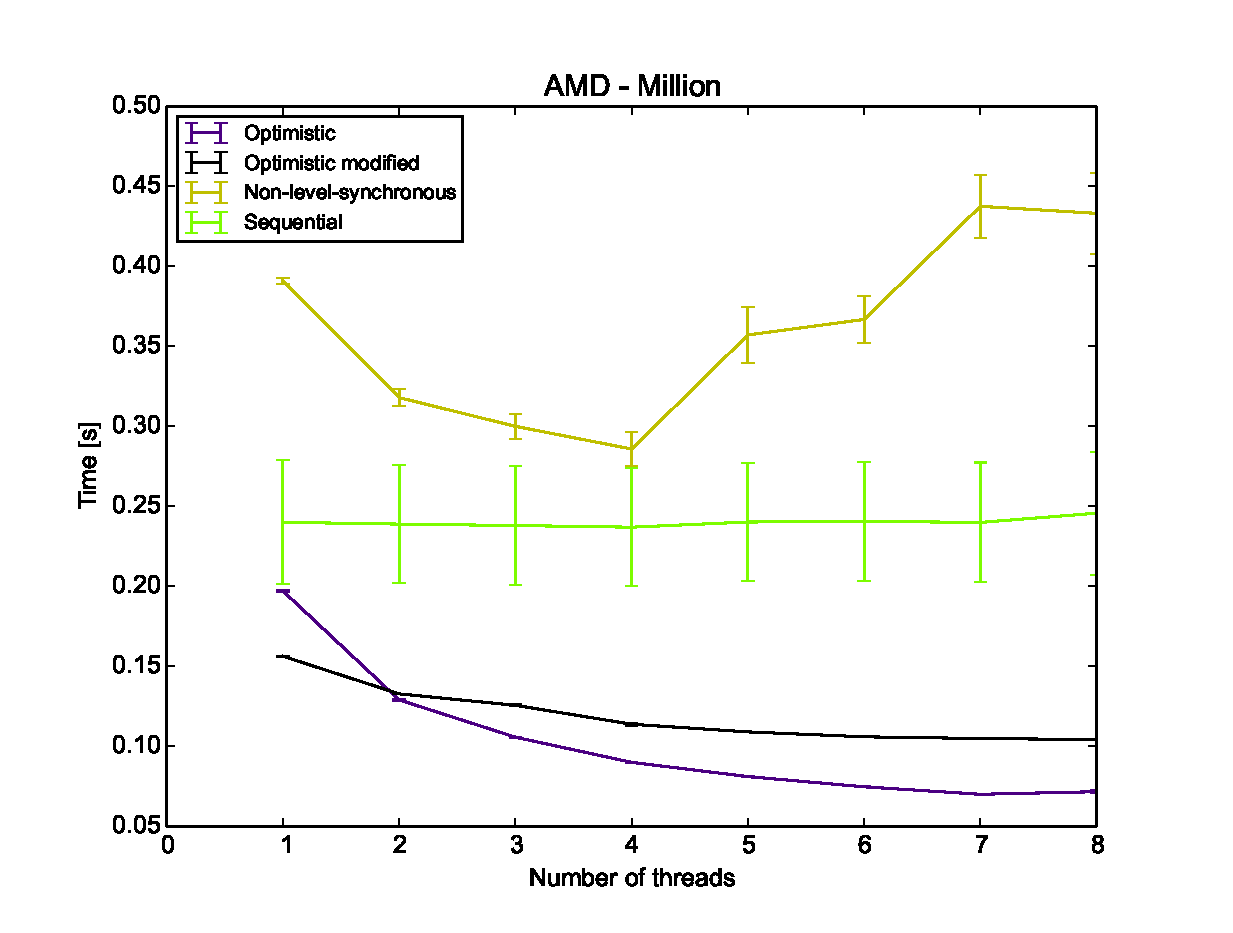
\includegraphics[width=0.9\textwidth]{amd_million.eps}
	  			\vspace*{-0.3cm}
	  			\caption[caption]{Performance of our BFS implementations on the \\ \hspace{\textwidth} AMD test environment operating on the Million graph.\label{fig:amdbig}}
			\end{minipage}%
			\begin{minipage}{.5\textwidth}
				\centering
	  			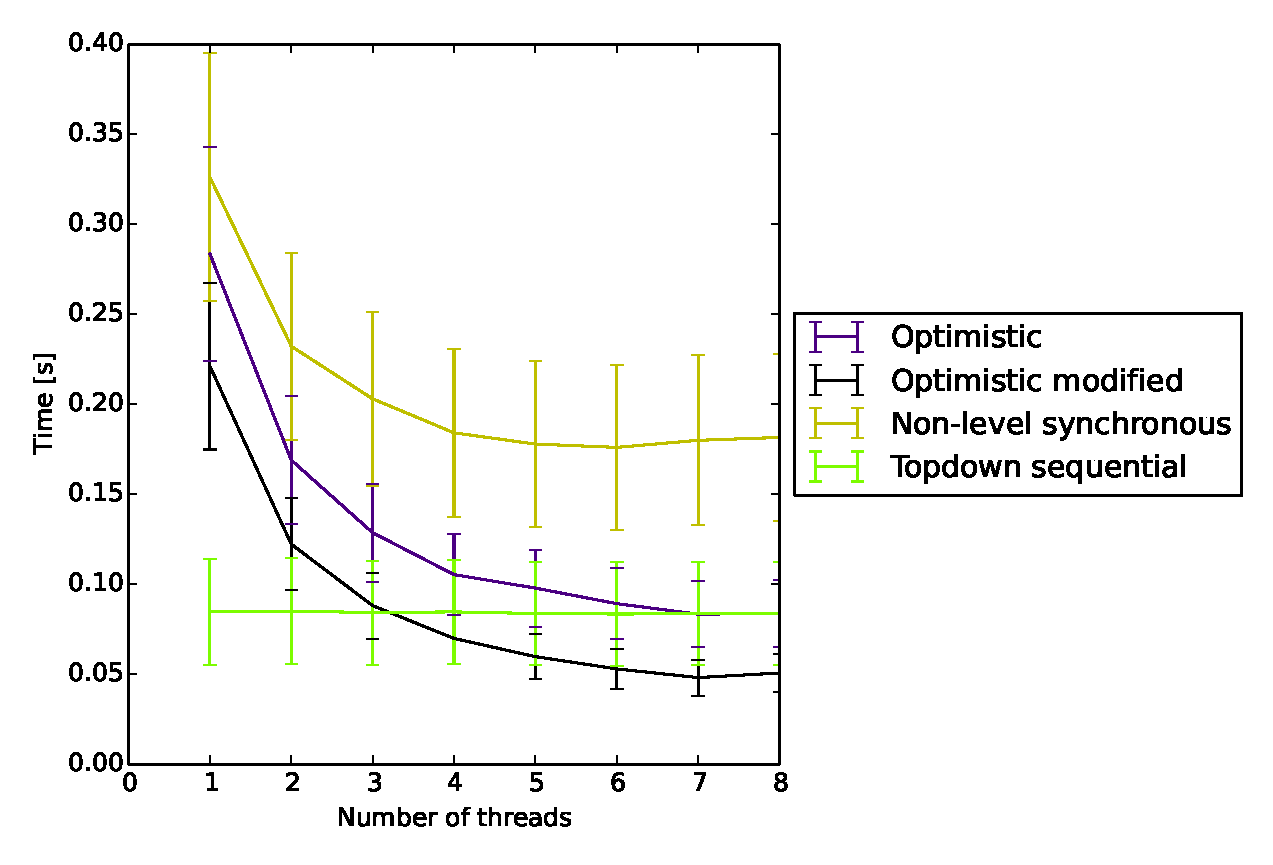
\includegraphics[width=0.9\textwidth]{amd_dimacskron.eps}
	  			\vspace*{-0.3cm}
	  			\caption[caption]{Performance of our BFS implementations on the \\ \hspace{\textwidth} AMD operating on the DIMACS Kronecker graph.\label{fig:amdkron}}
			\end{minipage}%
		\end{figure*}
		
		\begin{figure*}
			\centering
			\begin{minipage}{.5\textwidth}
				\centering
	  			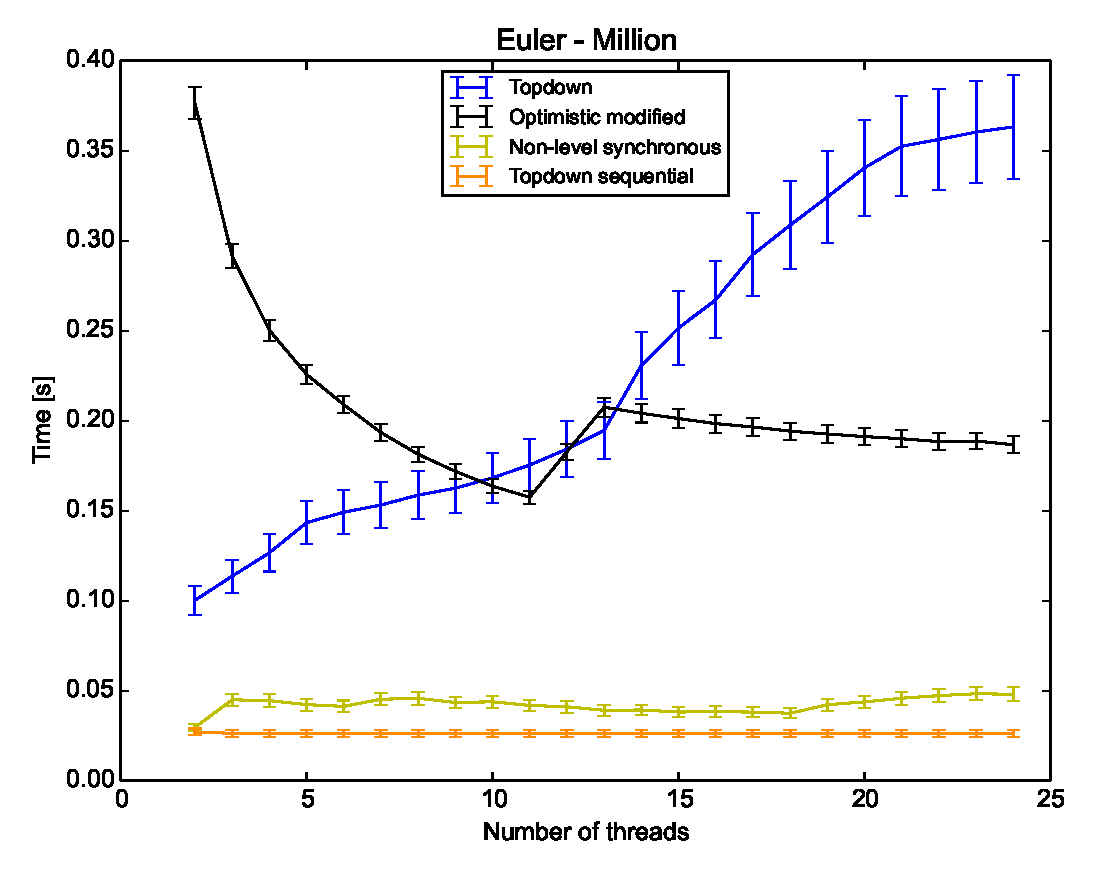
\includegraphics[width=0.8\textwidth]{euler_million.eps}
	  			\vspace*{-0.3cm}
	  			\caption[caption]{Performance of our BFS implementations on the \\ \hspace{\textwidth} Euler operating on the Million graph.\label{fig:eulerbig}}
			\end{minipage}%
			\begin{minipage}{.5\textwidth}
				\centering
	  			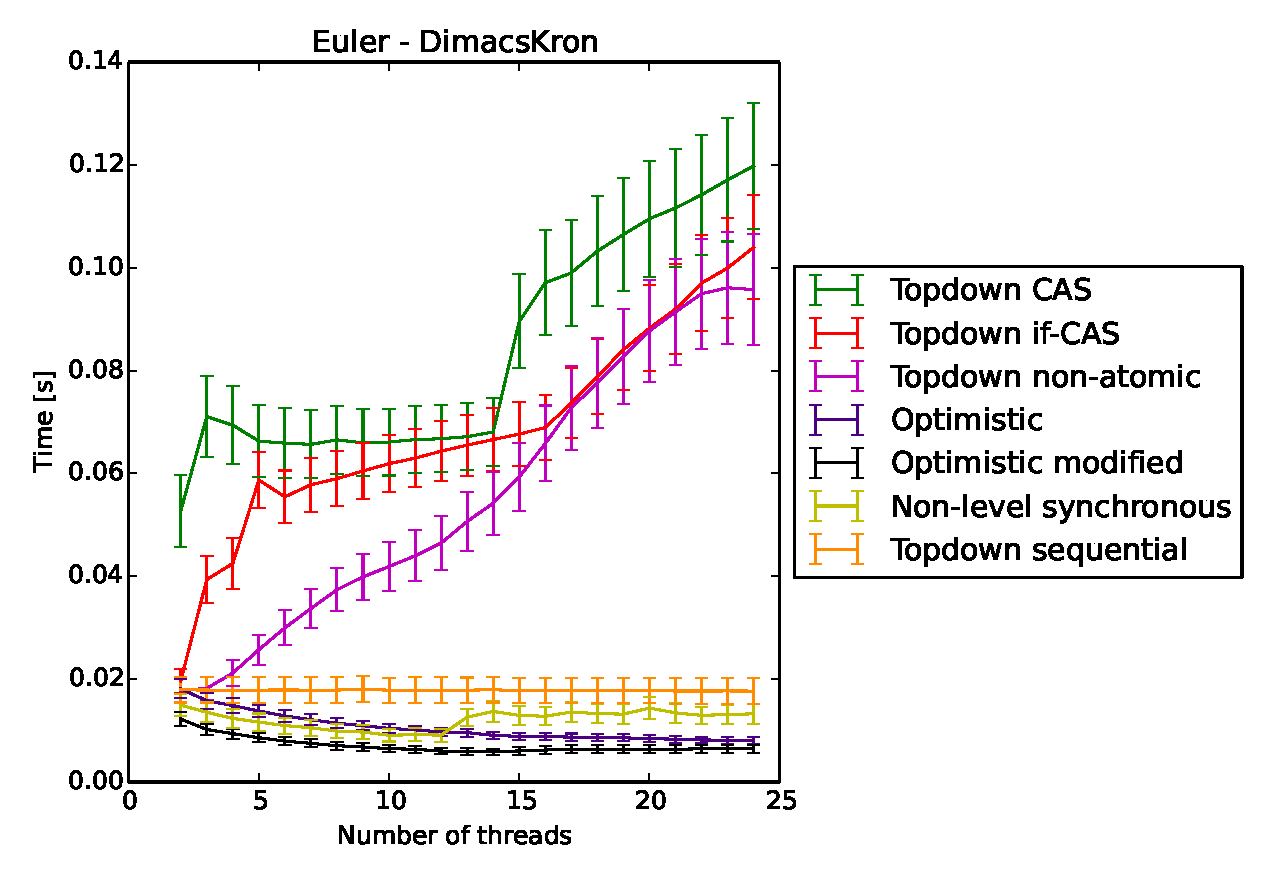
\includegraphics[width=0.8\textwidth]{euler_dimacskron.eps}
	  			\vspace*{-0.3cm}
	  			\caption[caption]{Performance of our BFS implementations on the \\ \hspace{\textwidth} Euler operating on the DIMACS Kronecker graph.\label{fig:eulerkron}}
			\end{minipage}%
		\end{figure*}

		\begin{figure*}
			\centering
			\begin{minipage}{.5\textwidth}
				\centering
	  			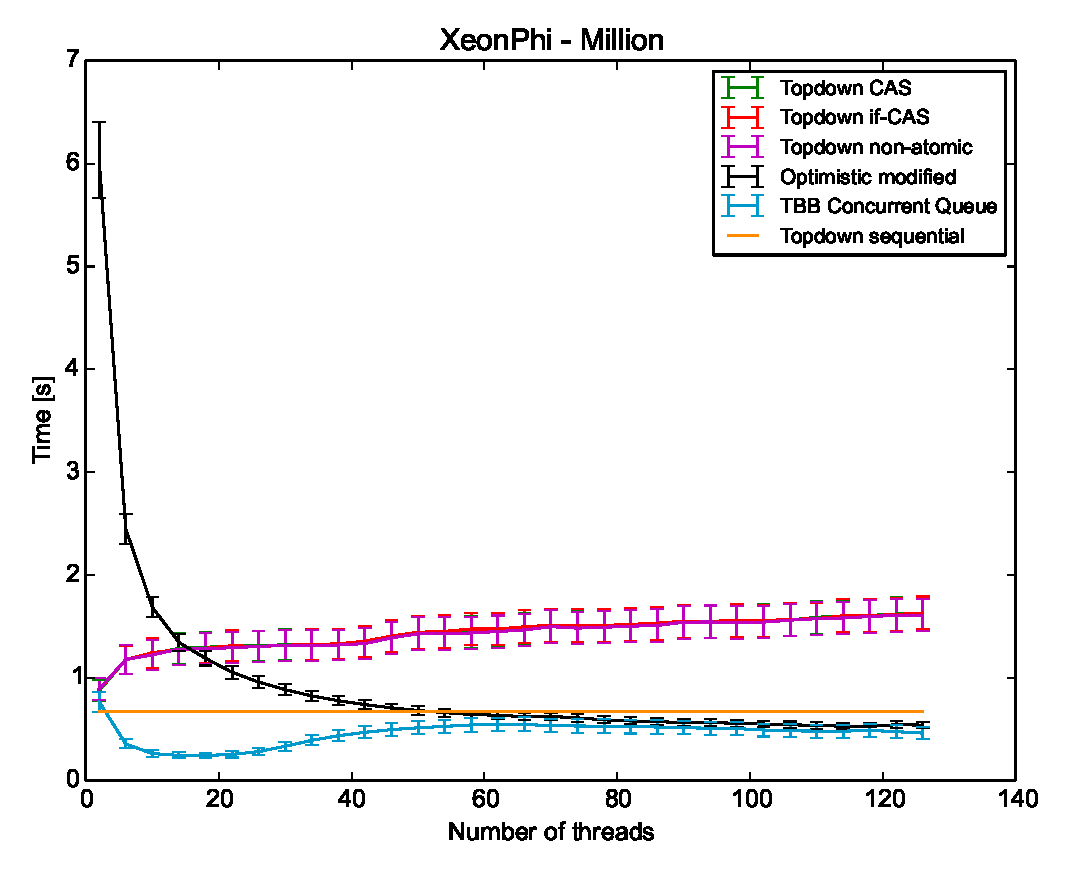
\includegraphics[width=0.8\textwidth]{einstein_million.eps}
	  			\vspace*{-0.3cm}
	  			\caption[caption]{Performance of our BFS implementations on the \\ \hspace{\textwidth} Einstein operating on the Million graph.\label{fig:einsteinbig}}
			\end{minipage}%
			\begin{minipage}{.5\textwidth}
				\centering
	  			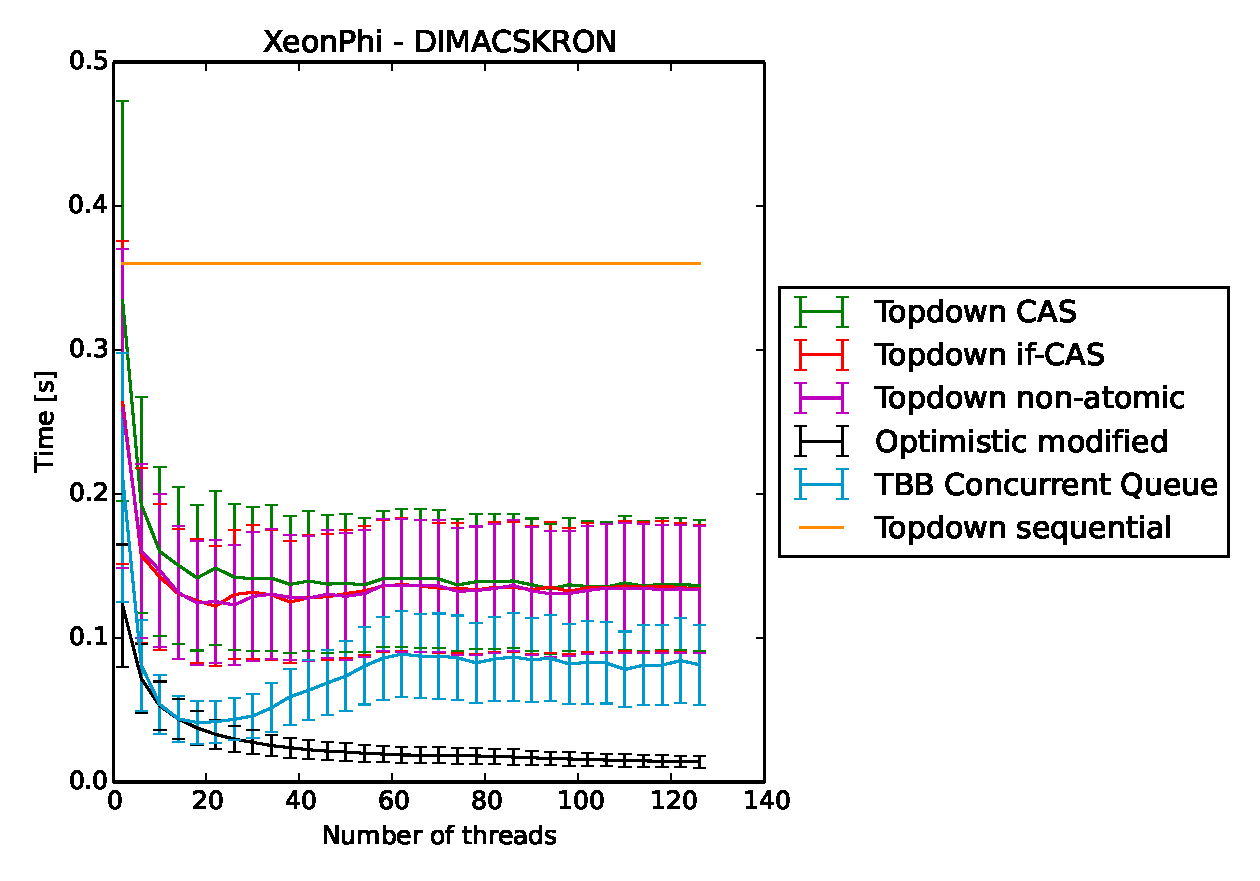
\includegraphics[width=0.8\textwidth]{einstein_dimacskron.eps}
	  			\vspace*{-0.3cm}
	  			\caption[caption]{Performance of our BFS implementations on the \\ \hspace{\textwidth} Einstein operating on the DIMACS Kronecker graph.\label{fig:einsteinkron}}
			\end{minipage}%
		\end{figure*}
		
%		\begin{figure}[t]
%			\centering
%	  		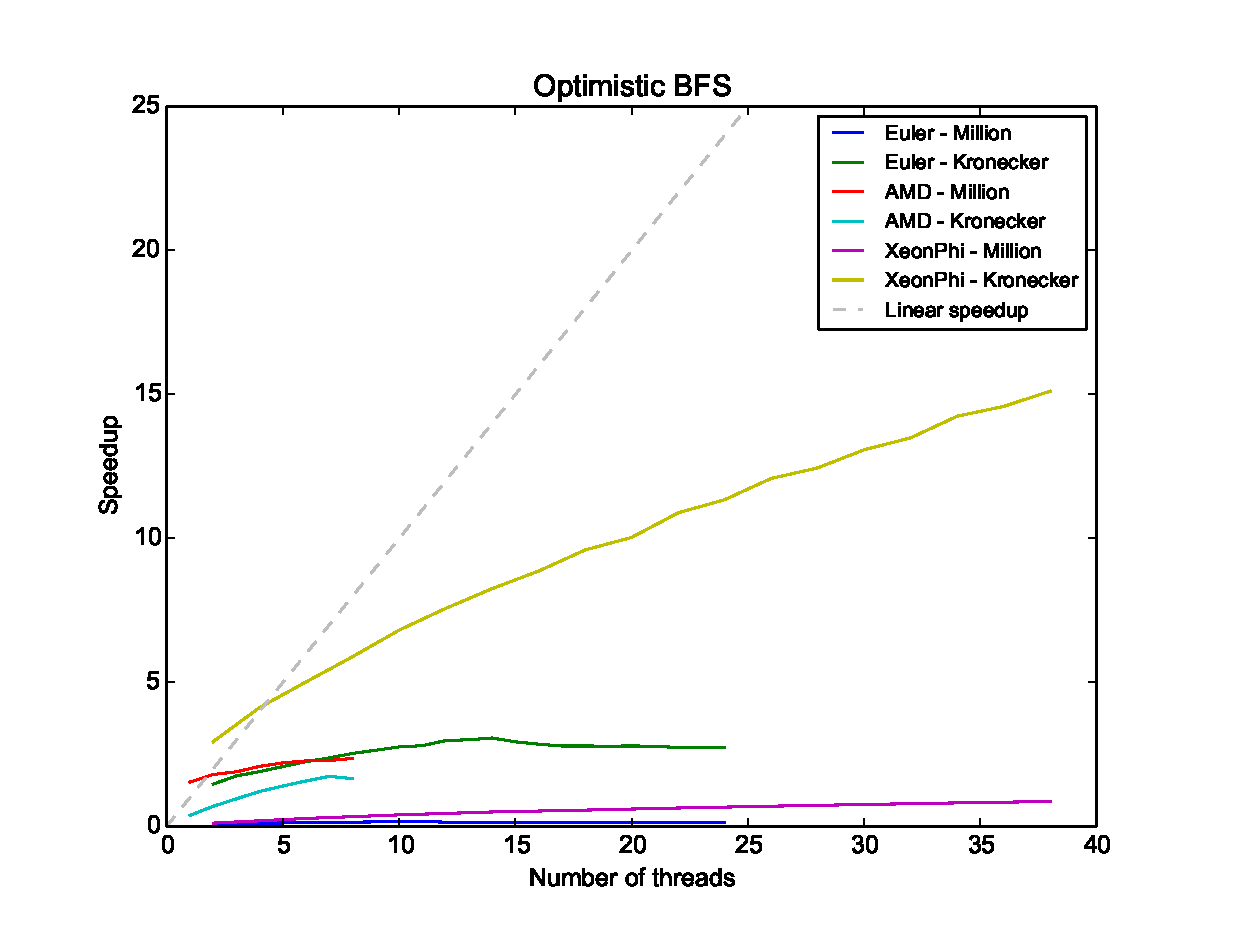
\includegraphics[scale=0.33]{optimistic_speedup.eps}
%	  		\vspace*{-0.3cm}
%	  		\caption{Speedup of Optimistic BFS on all platforms and graphs.\label{fig:speedup}}
%		\end{figure}


		In the following plots resulting from our experiments, not all version or approaches mentioned before appear on each of the test platforms. 
		The reason behind this is that some are too slow on one test environment while doing okay on another one.
		Versions omitted from a plot can therefore be assumed slower than any of the shown algorithms.
		
		In the experiments, multiple BFS started from different source vertices are averaged for every number of threads. 
		These measured average times, as well as their standard deviation, are shown in each plot.
		The goal of these experiments is to find the best performing algorithm and to see how different approaches behave in the case of strong scaling.

		First, we take a look at the AMD system.
		In Fig. \ref{fig:amdbig} we can observe the irregular and bad performance of the non-level-synchronous approach for the Million graph.
		In contrast, the Optimistic versions behave quite nicely and scale in an expected way.
		Running the Kronecker graph on the same system results in quite different results, as shown in Fig. \ref{fig:amdkron}.
		While the general behaviour of all shown algorithms seems okay, the cost of doing the BFS in parallel actually makes even the best version slower than the sequential solution up to 3 threads.
		With more than 3 threads we can see some speedup. 
		
		Switching to the Euler system with a higher number of maximal threads, we observe quite surprising results, see Fig. \ref{fig:eulerbig}.
		The biggest surprise is that for the Million graph, none of the implemented algorithms manages to be better than a simple sequential run.
		Reasons for this might be the small number of edges in this graph limiting the potential for parallel execution to a point where the cost for doing any synchronization or the additional work created to circumvent synchronization on this system is too great.

		Supporting this theory is the fact that in Fig. \ref{fig:eulerkron} we can see that for a more connected graph a few algorithms are an improvement in comparison to a sequential run.
		The main result from this experiment is the observation that any version that relies on \verb+OMP critical+, even if only to manipulate the used data structure, does not perform in a useful way.
		As a minor detail, the jump in the non-level-synchronous version in this plot or more clearly the jump for the Optimistic modified version in Fig. \ref{fig:eulerbig} between 12 and 13 threads can be explained as the switch from physical cores to hyperthreading.

		Lastly, on the Einstein system, where the Intel TBB library was available, we can compare the performance of a concurrent data structure approach with our Optimistic algorithm.
		In Fig. \ref{fig:einsteinbig} we can notice that on this system, it requires a lot more threads for the Optimistic approach to become useful. On the other hand, the TBB concurrent queue performs well for a limited number of threads, after which it loses performance with increasing number of threads.
		
		The same observation, though in less extremely, can be made for the Kronecker graph in Fig. \ref{fig:einsteinkron}, where the TBB concurrent queue is already much sooner outperformed by the Optimistic algorithm.


	\section{Discussion}\label{sec:disc} % Roughly column. + ~1-2 references + 1 table
		We now provide an analysis of the results of the experimental evaluation of Optimistic BFS and the other variants to achieve additional insight on the base of the conducted study.
		We would like to note that the study can't be considered as complete and additional experiments and analysis need to be conducted to achieve clear understanding of all the properties of the proposed algorithm.  
		Particularly, weak scaling experiments need to be conducted and dependencies of BFS performance on the target environment properties and target graph properties should be evaluated. 
		
		%Using the results of our experiments, we determined that the performance of a particular BFS implementation heavily depends on two major groups of factors. <- unnecessary
		One of the very general conclusions from the our study is that performance characteristics of memory intensive parallel algorithms depend heavily on the specifics of the target environment, i.e. its underlying hardware architecture, operating system and compiler.
		%To understand what components of the environment play a major role on the algorithm performance characteristics, additional experiments need to be conducted. <- mentioned just a paragraph before
		What we can see is that even on so similar hardware platforms like the AMD and Intel based implementations of an IA-32 architecture, the algorithm can demonstrate significantly different behaviour, which is surprising.
		What we can expect is that a parallel BFS algorithm which is optimal for all SMA architectures cannot exist at all and an algorithm must be developed and evaluated for a particular environment to achieve the best results.
		%Simple code reuse may not work if performance is really an issue. -> repeating the statement above
		
		This analysis also highlights the dependency of the performance of the variants of parallel BFS on the characteristics of the target graph, however it is not clear what exact characteristics affect the performance of Optimistic BFS and how they do so. 
		But detailed understanding of these dependencies and knowledges of the characteristics of typical graphs used in particular applications can help in the development of the best performing algorithm for this application.
		
		
		
	\section{Summary and Conclusion}\label{sec:suco} % Roughly half a column.
		In this paper we present the design, implementation, and evaluation of Optimistic BFS, a parallel version of breadth-first search for shared memory architectures.
		
		We demonstrate through experiments that this algorithm and the approach on synchronization avoidance outperforms in many cases not only approaches relying on cheap synchronization methods, but also approaches focused on improvement of load balancing. 		
		In fact, we observe that the even cheap synchronization methods can be very destructive for the performance and scalability of the algorithm.  
		Almost complete avoidance of synchronization results in a significant improvement of the performance of BFS. % and determinism <- ?
		
		In our experimental evaluation, we found that the level of optimality of BFS algorithms heavily depends on characteristics of the target environment and on characteristics of the target graph. % , including CPU architecture, operating system and compiler used, -> already mentioned in detail in the discussion section.
		
		In future work, it would be of interest to figure out what component of the Euler test environment is a main source of performance degradation of Optimistic BFS and thus find for which set of target environments it would be most optimal.  		
		It also would be interesting to figure out the relationships of the performance provided by optimistic BFS depending of different graph characteristics and hence find out for what class of graphs it would be most optimal.
		Furthermore, it will be beneficial to evaluate weak scaling properties of Optimistic BFS.
	
	\bibliographystyle 	{IEEEbib} % Roughly column. (10-15 references).
	\bibliography 		{bibl_conf}
\end{document}

